
%%% Variables de frecuencia por cada base de datos. 
\newcommand{\acm}{518}
\newcommand{\ieee}{0}
\newcommand{\sd}{120}
\newcommand{\spr}{209}
\newcommand{\tf}{0}
\newcommand{\tot}{847}
%%% Variables de contrubución porcetual
\newcommand{\acmp}{\fpeval{round(\acm*100/\tot,2)}}
\newcommand{\ieeep}{\fpeval{round(\ieee*100/\tot,2)}}
\newcommand{\sdp}{\fpeval{round(\sd*100/\tot,2)}}
\newcommand{\sprp}{\fpeval{round(\spr*100/\tot,2)}}
\newcommand{\tfp}{\fpeval{round(\tf*100/\tot,2)}}

%%%%% ------------------------------------------------

%%% Variables de frecuencia por cada base de datos. 
\newcommand{\iacm}{315}
\newcommand{\iieee}{0}
\newcommand{\isd}{101}
\newcommand{\ispr}{63}
\newcommand{\itf}{0}
\newcommand{\itot}{479}
%%% Variables de contribución porcentual
\newcommand{\iacmp}{\fpeval{round(\iacm*100/\itot,2)}}
\newcommand{\iieeep}{\fpeval{round(\iieee*100/\itot,2)}}
\newcommand{\isdp}{\fpeval{round(\isd*100/\itot,2)}}
\newcommand{\isprp}{\fpeval{round(\ispr*100/\itot,2)}}
\newcommand{\itfp}{\fpeval{round(\itf*100/\itot,2)}}

%Cantidad de estudios excluídos por ser duplicados
\newcommand{\numEstEx}{3}

%Cantidad de estudios luego de depuración = (estudios totales luego de exclusión - estudios duplicados)
\newcommand{\depTot}{\fpeval{\itot-\numEstEx}}

%Cantidad de estudios depurados por el screening
\newcommand{\screen}{377}
%Cantidad de estudios totales luego del screening
\newcommand{\screenTot}{\fpeval{\depTot-\screen}}

%sub-subseccion 4.2.2
\subsubsection{Search Strategy 1: Databases}

This strategy comprises two components. The first component is termed ``Study Identification''. It focuses on establishing the keywords to construct search strings that enable the completion of queries in digital libraries. The second component is called ``Study Selection''. It focuses on applying various criteria to refine study search results and select those with the most significant value for the SMS\@

\bolditalic{Study Identification}: in order to ensure the feasibility of the SMS given administrative decisions and resource availability, it was decided to limit the number of databases to five, including ACM, IEEE Xplore, Springer, ScienceDirect, Taylor \& Francis. In this part of the process, it was necessary to establish the keywords used subsequently in the search strings for each of the databases. Again, we used the PICOC model as a methodological guide to identify key terms or phrases that serve this purpose. We refined these terms by including synonyms (See Table~\ref{table:picoc_keywords}).

% -------- Table : Keywords identified using PICOC model. ------------
\begin{table}[htbp]
	\centering
	\caption{Keywords identified using the PICOC model}
	\label{table:picoc_keywords}
	\renewcommand{\arraystretch}{1}  % Increase row height globally
	\begin{tabular}{p{1.8cm}p{6cm}}
		\toprule
		\textbf{Component}           & \textbf{Keywords}                                                                                                                                                                                                                                                    \\
		\midrule
		\textbf{Population}          & Universes, HTCondor, Distributed and parallel computing, HTC, Software development, Virtualization and microservices, Computer networks, Computational infrastructure, Artificial intelligence, Data analysis, Computational thinking, Research, Teaching, Industry. \\
		\addlinespace[0.8em]
		\textbf{Intervention}        & Identification and classification.                                                                                                                                                                                                                                   \\
		\addlinespace[0.8em]
		\textbf{Acceptance Criteria} &
		Documented project cases, compliance with inclusion and exclusion criteria, and appearance in selected databases.                                                                                                                                                                                   \\
		\addlinespace[0.8em]
		\textbf{Outcomes}            & Taxonomy that organizes works related to the population.                                                                                                                                                                                                             \\
		\addlinespace[0.8em]
		\textbf{Context}             & HTCondor universes, distributed and parallel computing domains, academic functions, research, teaching, industry.                                                                                                                                                    \\
		\bottomrule
	\end{tabular}
\end{table}
% --------------------------------------------------------------


The selected main keywords were \textit{HTCondor, HTC, Universe, Project, Research}. To broaden the research perspective, we used the Boolean operator ``OR'' to add synonyms to the main keywords.

Finally, the set of keywords selected for the construction of the search string are found in Table~\ref{table:database_search_keywords}.


% -------- Table : Keywords for database search ------------
\begin{table}[htbp]
	\centering
	\caption{Keywords for database search}
	\label{table:database_search_keywords}
	\renewcommand{\arraystretch}{1}  % Increase row height globally
	\begin{tabular}{p{1.4cm}p{6.4cm}}
		\toprule
		\textbf{Keyword}  & \textbf{Synonyms and related concepts}                     \\
		\midrule
		\textbf{HTCondor} & Condor                                                     \\
		\addlinespace[0.8em]
		\textbf{HTC}      & HPC, High Throughput Computing, High Performance Computing \\
		\addlinespace[0.8em]
		\textbf{Universe} & Execution Environment                                      \\
		\addlinespace[0.8em]
		\textbf{Project}  & Work                                                       \\
		\addlinespace[0.8em]
		\textbf{Research} & Teaching, Industry                                         \\
		\bottomrule
	\end{tabular}
\end{table}
% --------------------------------------------------------------





% -------- Table : Search strings used in databases ------------
\begin{table*}[htbp]
	\centering
	\caption{Search strings used in databases}
	\label{table:cadenas_de_busqueda}
	\renewcommand{\arraystretch}{1}  % Increase row height globally
	\begin{tabular}{p{3.2cm}p{11cm}p{2.5cm}}
		\toprule
		\textbf{Database}                 & \textbf{Search String}                                                                                                                                                                                              & \textbf{Fields} \\
		\midrule
		\textbf{ACM Full Text Collection} & ((HTCondor OR Condor) AND (HTC OR ``High Throughput Computing'' OR HPC OR ``High Performance Computing'') AND (Universe OR ``Execution Environment'') AND (Project OR Work) AND (Research OR Teaching OR Industry)) & All fields      \\
		\addlinespace[0.8em]
		\textbf{IEEE Xplore}              & ((HTCondor OR Condor) AND (HTC OR ``High Throughput Computing'' OR HPC OR ``High Performance Computing'') AND (Universe OR ``Execution Environment'') AND (Project OR Work) AND (Research OR Teaching OR Industry)) & All fields      \\
		\addlinespace[0.8em]
		\textbf{Springer}                 & ((HTCondor | Condor) + (HTC | ``High Throughput Computing'' | HPC | ``High Performance Computing'') + (Universe | ``Execution Environment'') + (Project | Work) + (Research | Teaching | Industry))                 & All fields      \\
		\addlinespace[0.8em]
		\textbf{ScienceDirect}            & (HTCondor OR Condor) (HTC OR ``High Throughput Computing'' OR HPC OR ``High Performance Computing'') (Universe OR ``Execution Environment'') (Project OR Work) (Research OR Teaching OR Industry)                   & All fields      \\
		\addlinespace[0.8em]
		\textbf{Taylor \& Francis}        & ((HTCondor OR Condor) AND (HTC OR ``High Throughput Computing'' OR HPC OR ``High Performance Computing'') AND (Universe OR ``Execution Environment'') AND (Project OR Work) AND (Research OR Teaching OR Industry)) & All fields      \\
		\bottomrule
	\end{tabular}
\end{table*}
% --------------------------------------------------------------


To direct this research toward the intersection of these two groups of terms, the Boolean operator ``AND'' was used. Once we identified the keywords, we continued constructing the search strings for the digital libraries using an iterative process. The iterative construction of search strings consists of performing a heuristic process with keywords, synonyms, and related concepts through the use of disjunctions and conjunctions that conform to the syntactic rules of each database considered in the automated search. Therefore, these strings vary according to the characteristics and functions of each database. See Table~\ref{table:cadenas_de_busqueda}.

After constructing the search strings, these were submitted to each database engine. Table~\ref{table:search_results} shows the set of results obtained. We identified a total of 847 studies preliminarily, with ACM being the largest contributor, delivering the greatest number of results compared to the other databases with \acmp\% of the results.


\begin{table*}[htbp]
	\centering
	\caption{Search string results}
	\label{table:search_results}
	\renewcommand{\arraystretch}{1}  % Increase row height globally
	\begin{tabular}{p{4.8cm}p{1.7cm}p{1.7cm}p{1.7cm}p{1.7cm}p{2cm}p{1.4cm}}
		\toprule
		\textbf{Criteria}                         & \textbf{ACM} & \textbf{IEEE} & \textbf{ScienceDirect} & \textbf{Springer} & \textbf{Taylor\&Francis} & \textbf{Total} \\
		\midrule
		\textbf{Search string with keywords only} & \acm{}       & \ieee{}       & \sd{}                  & \spr{}            & \tf{}                    & \tot{}         \\
		\addlinespace[0.8em]
		\textbf{Percentage contribution}          & \acmp{}\%    & \ieeep{}\%    & \sdp{}\%               & \sprp{}\%         & \tfp{}\%                 & 100\%          \\
		\bottomrule
	\end{tabular}
\end{table*}
% --------------------------------------------------------------




\bolditalic{Study Selection}: to refine the results obtained up to this point, we applied the inclusion and exclusion criteria defined in the planning stage. Table~\ref{table:search_results_exclusion} shows the results of this step. After applying this filter, the total number of studies obtained was \itot. According to the different databases consulted, ACM continues to have the most considerable contribution, with \iacmp\% of the studies.

%% Applying duplicate exclusion

From the \itot{} studies selected, three studies were excluded because they were duplicates. After this refinement, the total number of studies was \depTot{}. From this new dataset, a review step, known as \bolditalic{screening} was conducted, this procedure consists of verifying the title, abstract, and keywords of each study to determine if these are circumscribed within the research context, that is, if they are aligned with the objectives proposed for the SMS. The \textit{screening} process allowed us to discard \screen{} studies given that some of them made reference to different academic disciplines and others were not aligned with the research objectives proposed.

Therefore, we concluded the first search strategy with a total of \screenTot{} studies selected. Figure~\ref{fig:overview} shows an overview of the activities and results obtained in search strategy 1.

\begin{figure}[htbp]
	\centering
	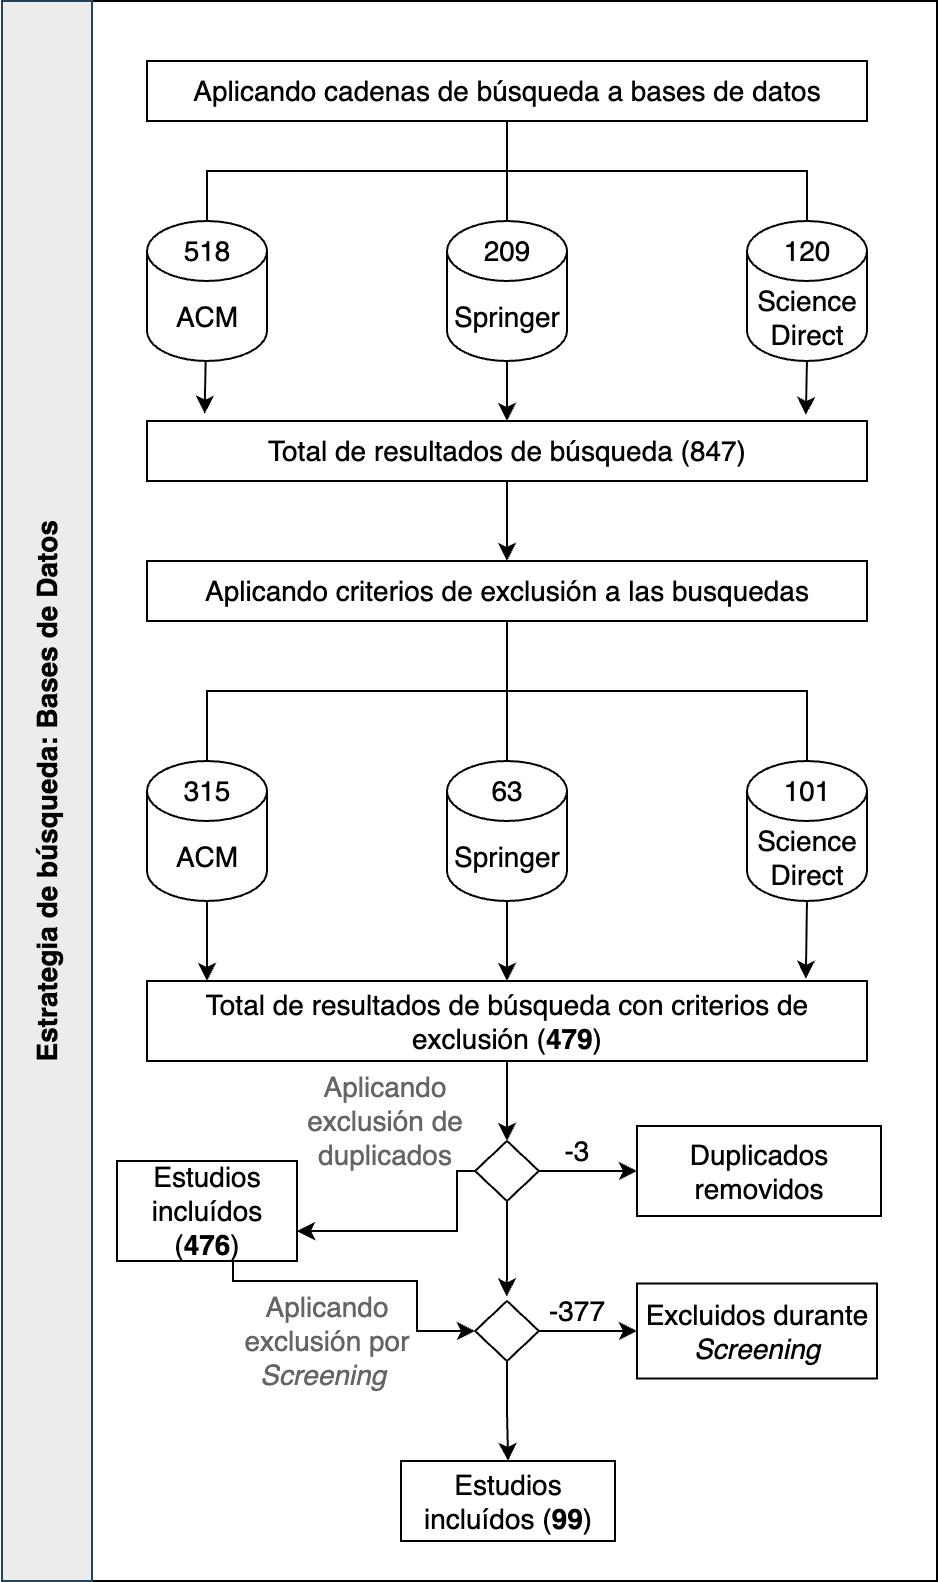
\includegraphics[scale=0.25]{resources/figures/overview.png}
	\caption{Overview of activities and results obtained in the database search strategy}
	\label{fig:overview}
\end{figure}


\begin{table*}[htbp]
	\centering
	\caption{Search string results with exclusion/inclusion criteria}
	\label{table:search_results_exclusion}
	\begin{tabular}{p{4.8cm}p{1.7cm}p{1.7cm}p{1.7cm}p{1.7cm}p{2cm}p{1.4cm}}
		\toprule
		\textbf{Criteria}                         & \textbf{ACM} & \textbf{IEEE} & \textbf{ScienceDirect} & \textbf{Springer} & \textbf{Taylor \& Francis} & \textbf{Total} \\
		\midrule
		\textbf{Search string with keywords only} & \iacm{}      & \iieee{}      & \isd{}                 & \ispr{}           & \itf{}                     & \itot{}        \\
		\addlinespace[0.8em]
		\textbf{Percentage contribution}          & \iacmp{}\%   & \iieeep{}\%   & \isdp{}\%              & \isprp{}\%        & \itfp{}\%                  & 100\%          \\
		\bottomrule
	\end{tabular}
\end{table*}
% --------------------------------------------------------------

